% Created 2022-03-30 Wed 16:38
% Intended LaTeX compiler: pdflatex
\documentclass[presentation,aspectratio=169]{beamer}
\usepackage[utf8]{inputenc}
\usepackage[T1]{fontenc}
\usepackage{graphicx}
\usepackage{grffile}
\usepackage{longtable}
\usepackage{wrapfig}
\usepackage{rotating}
\usepackage[normalem]{ulem}
\usepackage{amsmath}
\usepackage{textcomp}
\usepackage{amssymb}
\usepackage{capt-of}
\usepackage{hyperref}
\usepackage{khpreamble, euscript}
\DeclareMathOperator{\atantwo}{atan2}
\newcommand*{\ctrb}{\EuScript{C}}
\newcommand*{\obsv}{\EuScript{O}}
\usetheme{default}
\author{Kjartan Halvorsen}
\date{\today}
\title{El modelo canónico de robots móviles no-holonómicos}
\hypersetup{
 pdfauthor={Kjartan Halvorsen},
 pdftitle={El modelo canónico de robots móviles no-holonómicos},
 pdfkeywords={},
 pdfsubject={},
 pdfcreator={Emacs 26.3 (Org mode 9.4.6)}, 
 pdflang={English}}
\begin{document}

\maketitle

\section{Mobile robots}
\label{sec:orgb4c78bb}

\begin{frame}[label={sec:orgfc6503f}]{Modelo canónico a.k.a modelo uniciclo}
\begin{center}
 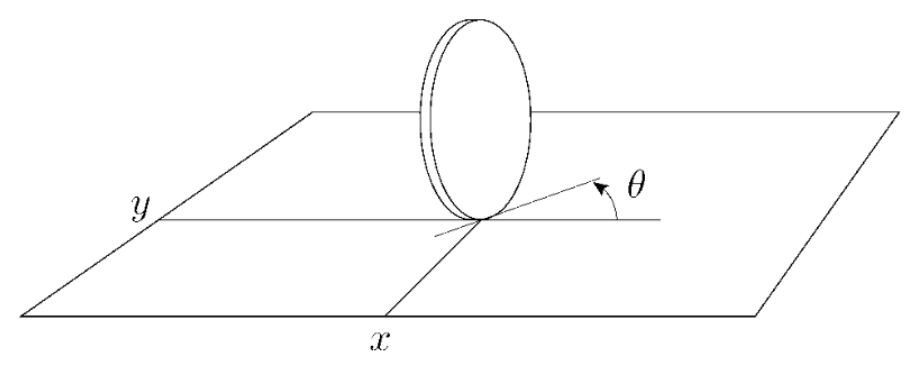
\includegraphics[width=.6\linewidth]{../figures/unicycle-kth.png}
\end{center}

\footnotesize
De Martina Zambelli (2013) \emph{Posture regulation for unicycle-like robots with prescribed performance guarantees}. KTH - Royal Institute of Technology, Sweden.
\end{frame}


\section{Differential drive}
\label{sec:org9c556a4}

\begin{frame}[label={sec:org093d6a7}]{Robot tipo diferencial (\emph{differential drive})}
\begin{center}
 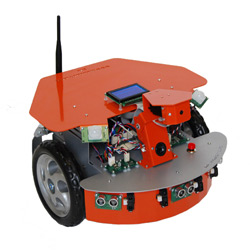
\includegraphics[width=.5\linewidth]{../figures/X80Pro.jpg}
\end{center}

X80Pro Dr. Robot Inc.
\end{frame}

\begin{frame}[label={sec:org3489ce1}]{Robot móvil - modelo uniciclo}
\begin{columns}
\begin{column}{0.4\columnwidth}
\begin{center}
 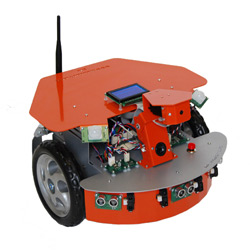
\includegraphics[width=.3\linewidth]{../figures/X80Pro.jpg}
\end{center}
\begin{center}
 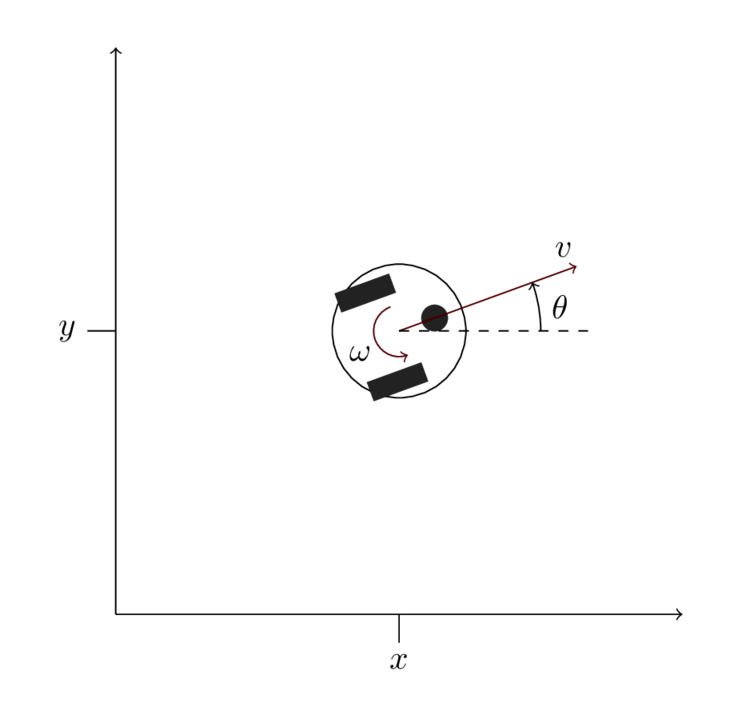
\includegraphics[width=1.0\linewidth]{../figures/unicycle-model}
\end{center}
\end{column}

\begin{column}{0.6\columnwidth}
\pause

\alert{Cinemática}

\[ \xi = \begin{bmatrix} \theta\\x\\y \end{bmatrix},   \quad u = \begin{bmatrix} \omega\\v \end{bmatrix}\]



\[\frac{d}{dt} \xi = \begin{bmatrix} \dot{\theta}\\\dot{x}\\\dot{y} \end{bmatrix} = \begin{bmatrix} \omega\\ v\cos\theta\\v\sin\theta\end{bmatrix} \]
\end{column}
\end{columns}
\end{frame}



\begin{frame}[label={sec:orga45f18e}]{Diferencial a modelo uniciclo}
\begin{columns}
\begin{column}{0.4\columnwidth}
\begin{center}
 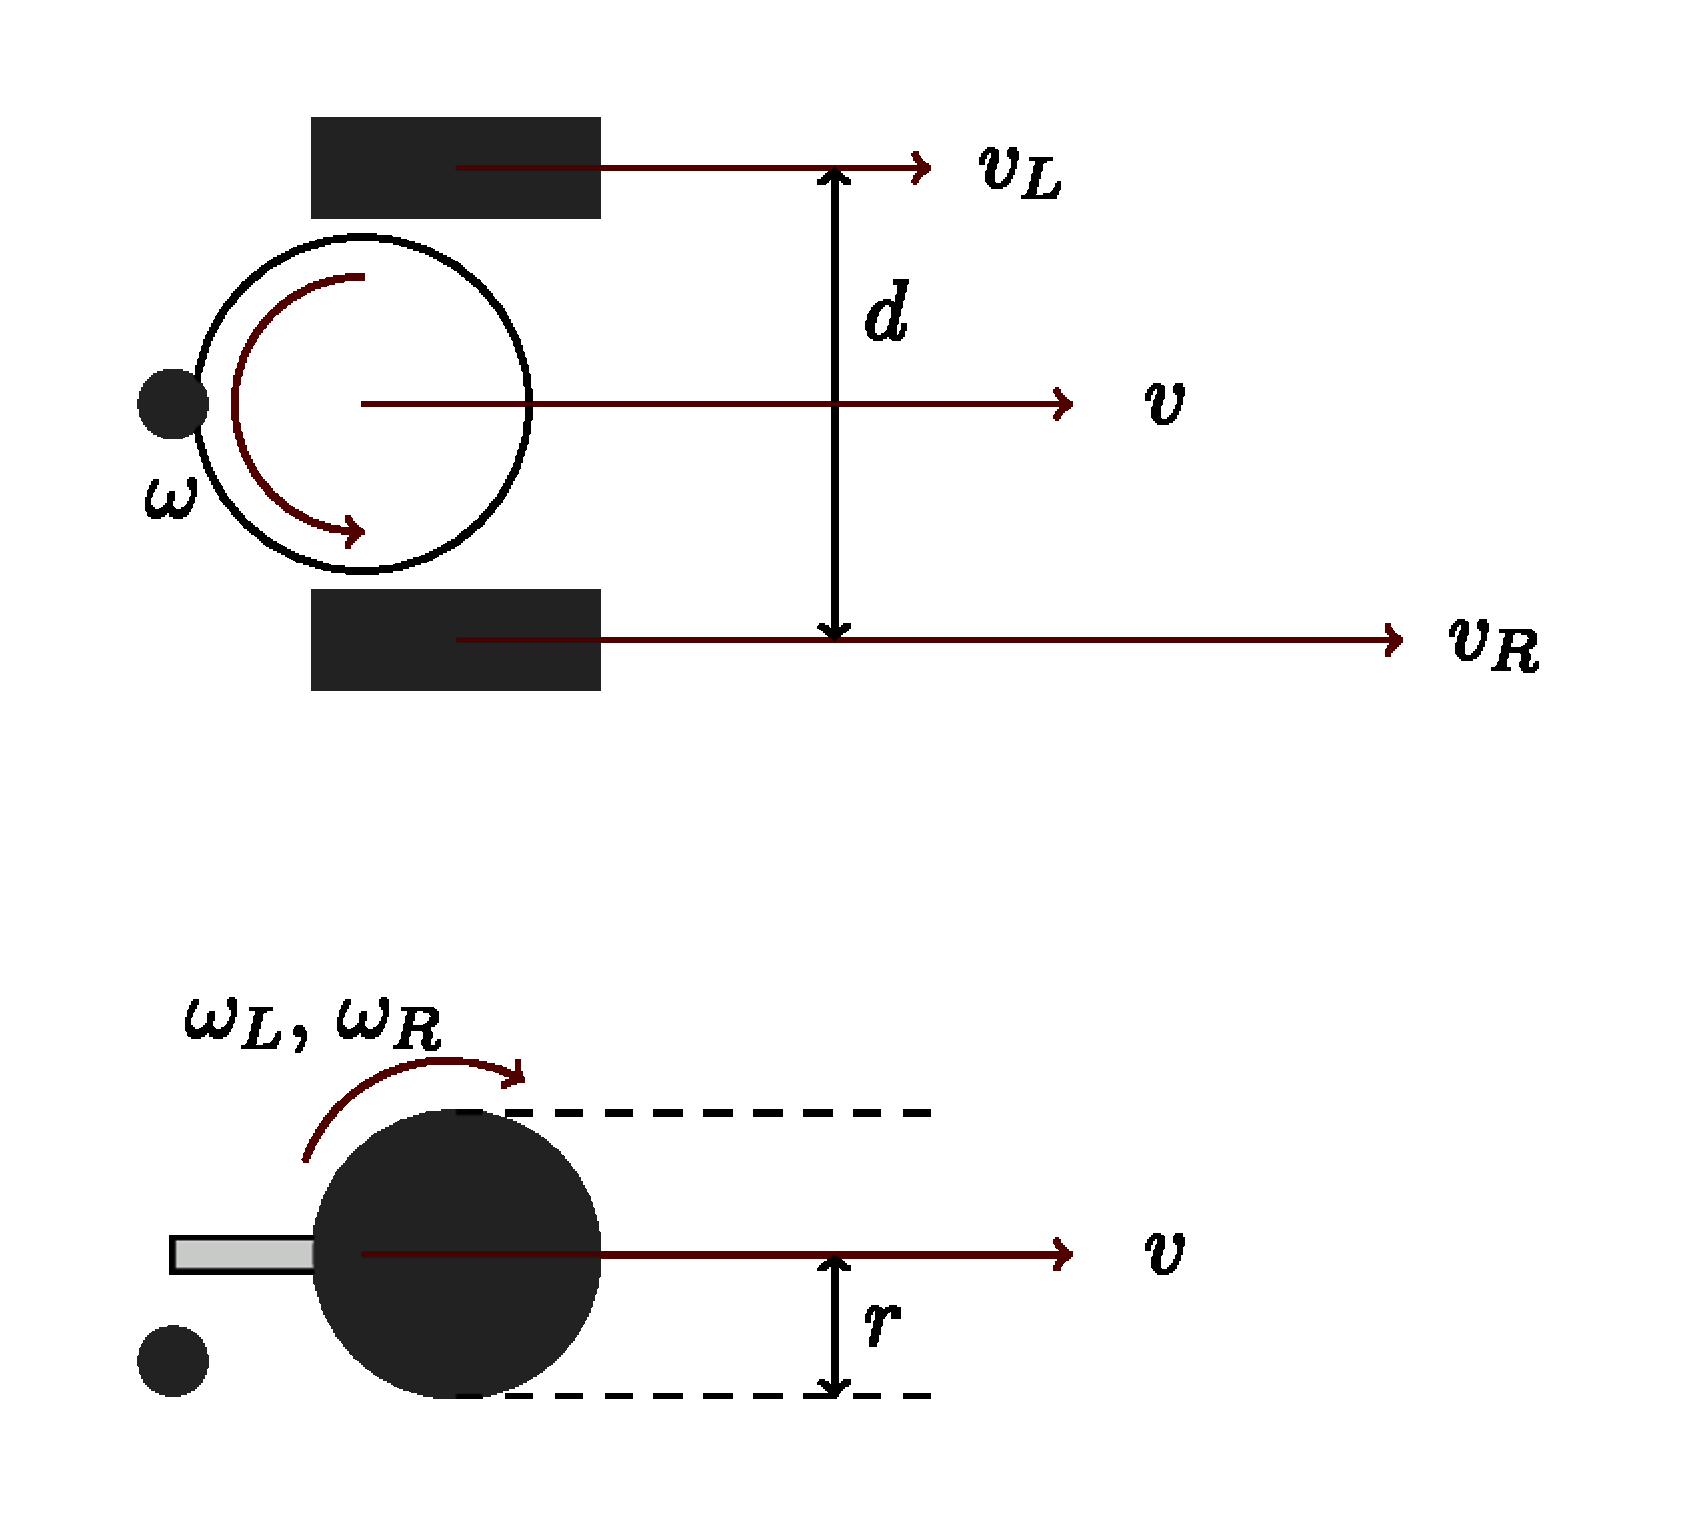
\includegraphics[width=1.0\linewidth]{../figures/unicycle-model-details}
\end{center}
\end{column}

\begin{column}{0.6\columnwidth}
\pause

\alert{Actividad} Determine

\begin{enumerate}
\item La velocidad lineal (\(v_R\), \(v_L\)) de cada rueda dado su velocidad angular (\(\omega_R\), \(\omega_L\))

\item La velocidad lineal \(v\) del centro robot dado las dos velocidades \(v_R\) y \(v_L\)

\item La velocidad angular \(\omega\) del robot dado las dos velocidades \(v_R\) y \(v_L\)

\item Las relaciones invertidas. Es decir, las velocidades angulares \(\omega_R\) y \(\omega_L\) de los ruedos dado las velocidades \(v\) y \(\omega\).
\end{enumerate}
\end{column}
\end{columns}
\end{frame}


\begin{frame}[label={sec:org7af4ead}]{Diferencial a modelo uniciclo}
\begin{columns}
\begin{column}{0.4\columnwidth}
\begin{center}
 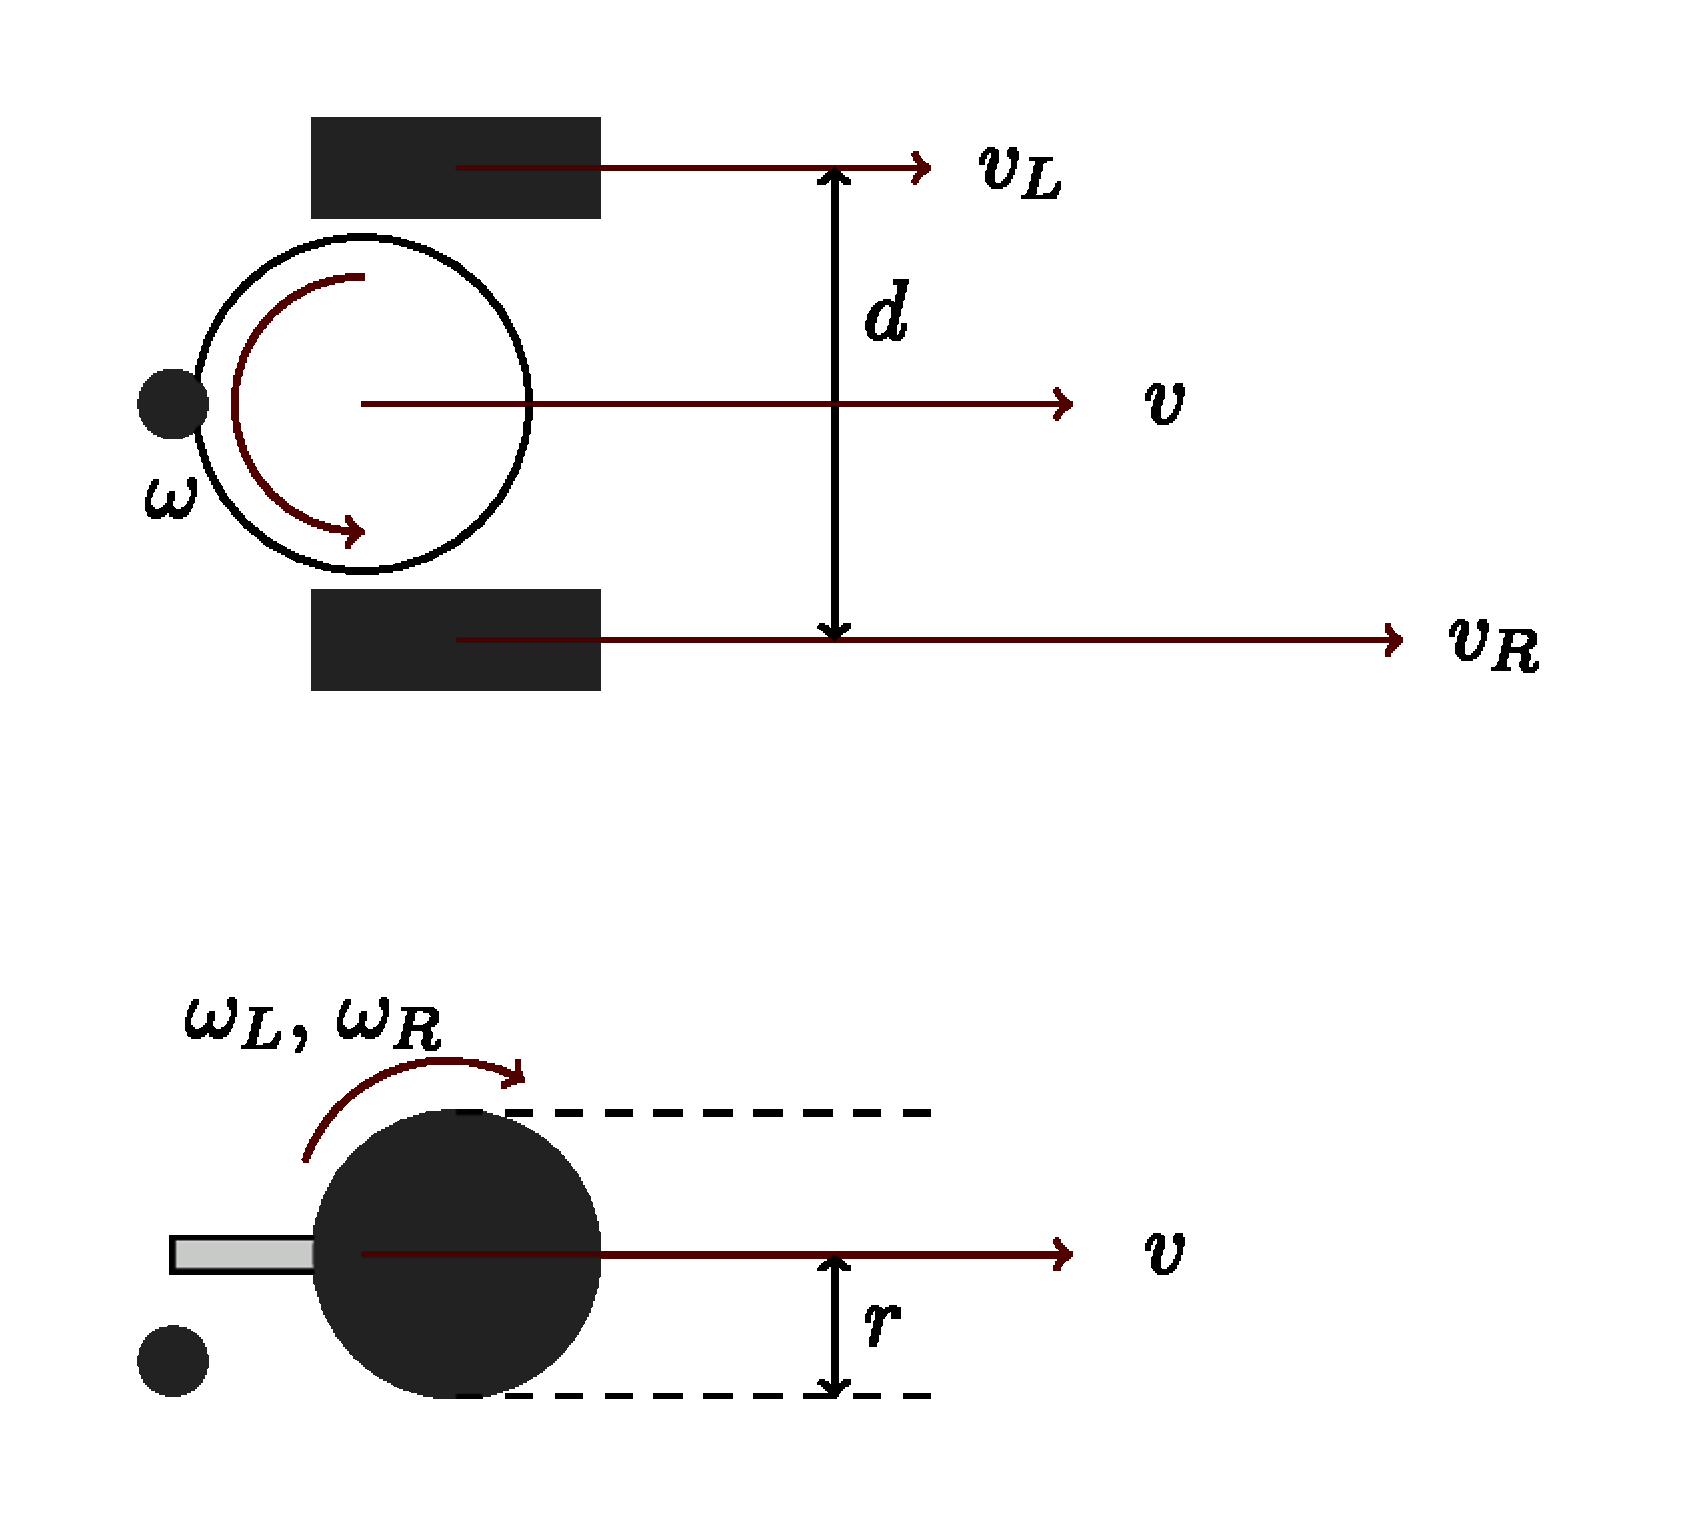
\includegraphics[width=.8\linewidth]{../figures/unicycle-model-details}
\end{center}
\end{column}

\begin{column}{0.6\columnwidth}
Asumiendo simetría entre las dos ruedas y en la dirección de giro.

\[ \omega_L,\, \omega_R \; \in \; [-\omega_{max}, \omega_{max}]\]

\pause

\alert{Actividad}
Dibuje la región de posibles valores de la señal de entrada al modelo canónico,
\[ u(t) = \begin{bmatrix} \omega(t)\\v(t) \end{bmatrix}, \]
dado los límites de la velocidad angular de las ruedas.
\end{column}
\end{columns}
\end{frame}


\begin{frame}[label={sec:org4f686c1}]{Implementación}
Notebook en google colab (página en Canvas)
\end{frame}


\section{Car-like}
\label{sec:org2cd4728}

\begin{frame}[label={sec:org1421399}]{Robots tipo coche - modelo bicicleta}
\begin{columns}
\begin{column}{0.4\columnwidth}
\begin{center}
 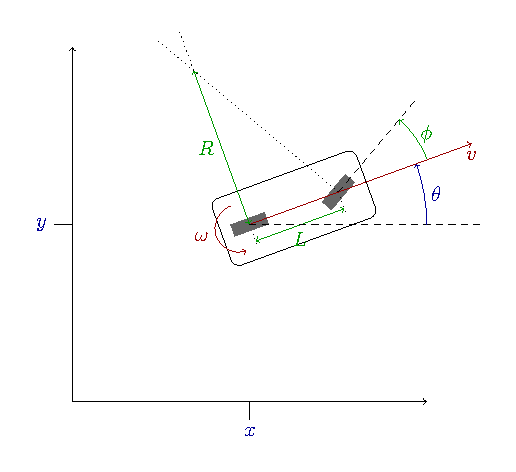
\includegraphics[width=1.05\linewidth]{../figures/bicycle-model}
\end{center}
\end{column}

\begin{column}{0.6\columnwidth}
\pause

Para un robot que se mueve instantaneamente en una trayectoria círcular con radie \(R\), la relación entre la velocidad lineal \(v\) y la velocidad angular \(\omega\) es

\pause

\[ v = R\omega \quad \Rightleftarrow \quad \omega = \frac{1}{R} v \]

\pause
\alert{Actividad} Determine el radie de giro instantaneo \(R\) como función del ángulo de dirección \(\phi\).

\pause
\alert{Actividad} Determine la velocidad angular \(\omega\) como función de la velocidad \(v\) y del ángulo de dirección \(\phi\). Determine también la función inversa.
\end{column}
\end{columns}
\end{frame}




\begin{frame}[label={sec:orgbd0ef99}]{Robots tipo coche - modelo bicicleta}
\begin{columns}
\begin{column}{0.4\columnwidth}
\begin{center}
 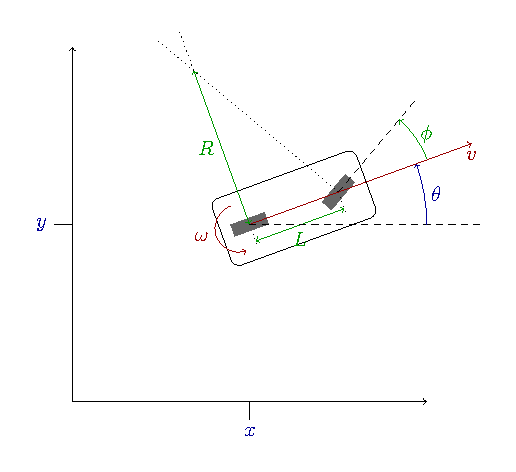
\includegraphics[width=1.05\linewidth]{../figures/bicycle-model}
\end{center}
\end{column}

\begin{column}{0.6\columnwidth}
Para cierto robot
\[ v \in [-v_{lm}, v_{um}], \quad \phi \in [-\phi_{max}, \phi_{max}]\]


\pause

\alert{Actividad} Dibuje la región de posibles valores de la señal de entrada al modelo canónico,
\[ u(t) = \begin{bmatrix} \omega(t)\\v(t) \end{bmatrix}, \]
dado los límites de la velocidad \(v\) y del ángulo de dirección \(\phi\).
\end{column}
\end{columns}
\end{frame}


\begin{frame}[label={sec:orgaf693a2}]{Implementación}
Notebook en google colab (página en Canvas)
\end{frame}
\end{document}